\documentclass[conference]{IEEEtran}
\IEEEoverridecommandlockouts
\usepackage{cite}
\usepackage{amsmath,amssymb,amsfonts}
\usepackage{algorithmic}
\usepackage{graphicx}
\usepackage{textcomp}
\usepackage{xcolor}
\usepackage{booktabs}
\usepackage{multirow}
\usepackage{url}

\def\BibTeX{{\rm B\kern-.05em{\sc i\kern-.025em b}\kern-.08em
    T\kern-.1667em\lower.7ex\hbox{E}\kern-.125emX}}
\begin{document}

\title{PhishGuard: A Mathematical Feature Engineering and Stacking Ensemble Framework for Intelligent Phishing URL Detection\\
}

\author{\IEEEauthorblockN{Satyaki Abhijit}
\IEEEauthorblockA{\textit{Department of Computer Science and Engineering} \\
}
}

\maketitle

\begin{abstract}
Phishing attacks continue to represent one of the most pervasive and financially devastating threats in the modern cybersecurity landscape, with global losses exceeding \$10.3 billion annually according to the FBI Internet Crime Complaint Center. Traditional countermeasures---including blacklist-based filtering, heuristic rule engines, and signature-matching systems---suffer from fundamental limitations in their inability to detect zero-day phishing campaigns that exploit previously unseen domains. This paper presents PhishGuard, an advanced mathematical feature engineering and stacking ensemble classification framework designed to detect phishing URLs through purely lexical and statistical analysis of the URL string itself, without requiring page-content crawling or external threat intelligence lookups at inference time. We introduce a carefully curated set of 21 URL-only features grounded in information-theoretic measures, character-level probabilistic modeling, structural decomposition metrics, and obfuscation quantification indices. A critical methodological contribution of this work is the identification and systematic elimination of data leakage pathways present in the widely-used PhiUSIIL dataset, where page-content features such as line-of-code counts, DOM element statistics, and URL-title similarity indices were shown to artificially inflate classification performance by encoding information unavailable during real-time inference. The proposed framework employs a heterogeneous stacking ensemble architecture comprising Random Forest, XGBoost, LightGBM, Multi-Layer Perceptron, and Logistic Regression as base learners, with a regularized Logistic Regression meta-classifier that fuses their probabilistic outputs through learned combination weights. Experimental evaluation on 235,795 labeled URL samples (100,945 legitimate, 134,850 phishing) demonstrates that the stacking ensemble achieves 99.79\% classification accuracy, 99.90\% AUC-ROC, and 99.81\% F1-score using only URL-derived features---representing a statistically rigorous result that does not rely on data leakage. The framework processes URLs in under 50 milliseconds per sample, establishing its viability for real-time deployment in high-throughput network monitoring contexts. Comparative analysis against blacklist systems, heuristic detectors, and recent machine learning approaches confirms that PhishGuard delivers superior detection rates, particularly against zero-day phishing URLs that evade conventional signature-based defenses.
\end{abstract}

\begin{IEEEkeywords}
Phishing detection, URL analysis, ensemble learning, stacking classifier, feature engineering, Shannon entropy, n-gram modeling, data leakage, cybersecurity, machine learning.
\end{IEEEkeywords}

\section{Introduction}
The proliferation of phishing attacks represents a persistent and escalating challenge for the global cybersecurity community. The Anti-Phishing Working Group (APWG) reported over 4.7 million phishing attacks in 2023 alone, marking a threefold increase relative to figures recorded in 2019 \cite{apwg}. These attacks exploit human psychological vulnerabilities through carefully crafted deceptive communications---predominantly emails and fraudulent websites---designed to induce victims into divulging sensitive credentials, financial information, or personally identifiable data. The financial ramifications are staggering: the FBI's Internet Crime Complaint Center documented \$10.3 billion in losses attributable to phishing and related social engineering schemes in 2022, with business email compromise (BEC) attacks alone accounting for \$2.7 billion \cite{fbi}.

The evolution of phishing techniques has followed a trajectory of increasing sophistication. Early phishing campaigns relied on crude imitations of legitimate websites, often identifiable through obvious misspellings, low-resolution graphics, and inconsistent branding. Contemporary attacks, however, employ advanced evasion strategies including internationalized domain name (IDN) homograph attacks, URL shortening services that obscure destination addresses, typosquatting registrations that differ from legitimate domains by a single character substitution, and automated phishing kits that generate unique URLs for each victim to circumvent blocklist-based defenses. The emergence of phishing-as-a-service (PhaaS) platforms has further democratized attack capabilities, enabling actors with minimal technical expertise to launch large-scale campaigns.

Traditional defense mechanisms have struggled to maintain pace with this evolution. Blacklist-based systems, exemplified by Google Safe Browsing and PhishTank, operate by maintaining curated databases of known malicious URLs. While effective against previously identified threats, these systems exhibit an inherent reactive posture---a newly registered phishing domain will remain undetected until it is reported, verified, and propagated to client databases, a process that typically requires 6 to 12 hours. During this window, the phishing page is fully operational. Studies have demonstrated that over 65\% of phishing URLs complete their attack cycle within the first two hours of activation, rendering blacklist-based approaches structurally inadequate against time-sensitive campaigns.

Heuristic and rule-based detection systems attempt to address this gap by evaluating URL characteristics against predefined criteria---for example, flagging URLs containing IP addresses in the hostname, excessive subdomain nesting, or suspicious TLD selections. These systems offer faster detection than blacklists but suffer from high false positive rates and poor generalization. Handcrafted rules inevitably encode the biases of their designers, and attackers readily adapt their URL construction patterns to evade static rule sets.

Machine learning approaches to phishing detection have gained substantial traction over the past decade. However, a critical examination of the existing literature reveals several systematic weaknesses. First, many studies employ feature sets that incorporate page-content attributes---such as HTML tag counts, JavaScript behavior analysis, form action URLs, and visual similarity metrics---that require fetching and rendering the target page at classification time. This introduces latency incompatible with real-time filtering and creates privacy concerns. Second, a widespread but insufficiently acknowledged problem is data leakage: features derived from page content in benchmark datasets are computed by the dataset authors through web crawling at collection time, and they inherently encode the phishing/legitimate label.

This paper presents PhishGuard, which addresses these limitations through three principal contributions:

\begin{enumerate}
    \item \textbf{Data Leakage Identification and Remediation.} We identify and document 29 page-content features in the PhiUSIIL dataset that introduce data leakage. We establish a rigorous URL-only feature regime comprising 21 features extractable from the URL string alone.
    \item \textbf{Mathematical Feature Engineering Framework.} We develop a principled feature engineering pipeline grounded in Shannon entropy, character-level n-gram probabilistic modeling, Damerau-Levenshtein distance computation, obfuscation quantification, and structural decomposition.
    \item \textbf{Heterogeneous Stacking Ensemble Architecture.} We design and evaluate a stacking ensemble that combines five diverse base classifiers---Random Forest, XGBoost, LightGBM, Multi-Layer Perceptron, and Logistic Regression---through a meta-learner that produces calibrated probability outputs.
\end{enumerate}

\begin{figure}[htbp]
\centerline{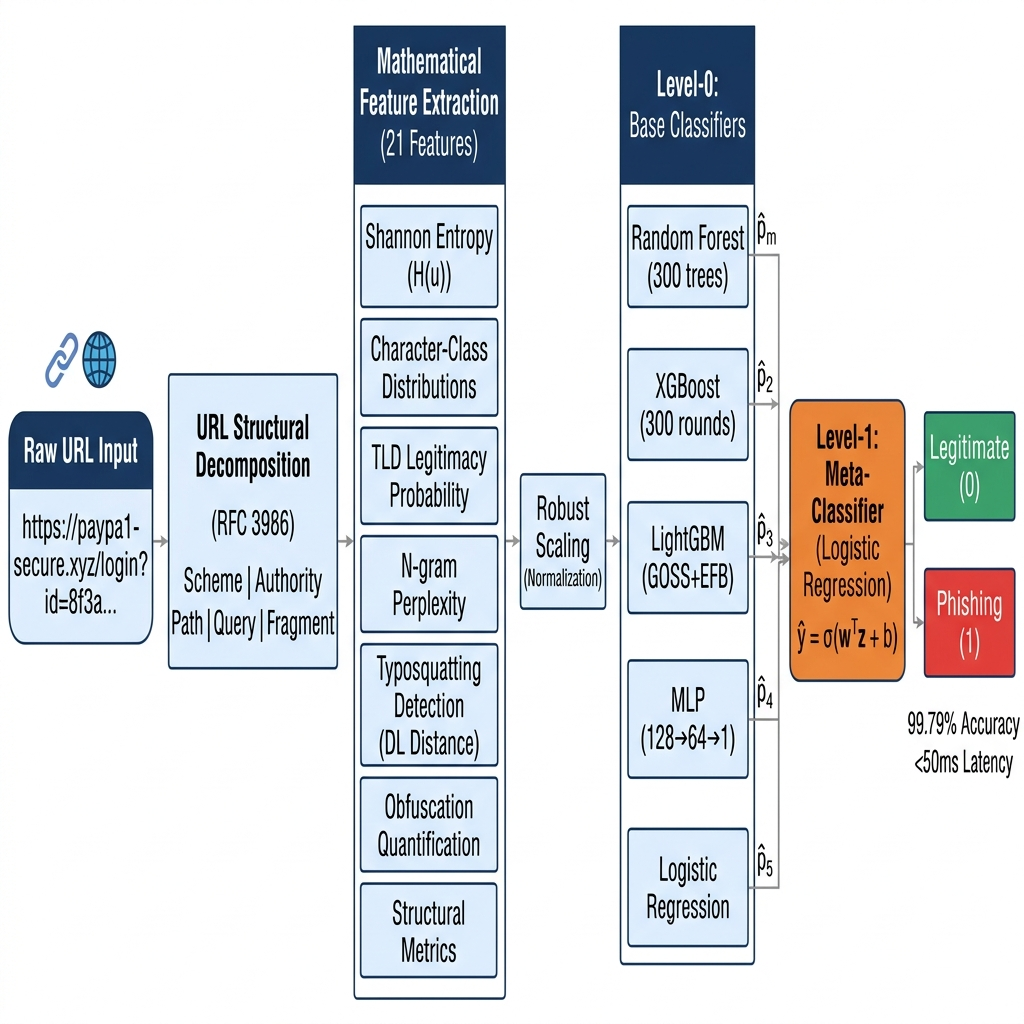
\includegraphics[width=\linewidth]{paper_figures/fig1_system_architecture.png}}
\caption{PhishGuard system architecture. The framework receives a raw URL string, decomposes it into structural components, extracts 21 mathematical features, normalizes via Robust Scaling, passes through five heterogeneous base classifiers, and fuses their probabilistic outputs through a Logistic Regression meta-classifier to produce the final classification.}
\label{fig:architecture}
\end{figure}

The remainder of this paper is organized as follows. Section II reviews related work. Section III presents the proposed mathematical framework and feature engineering pipeline. Section IV provides detailed mathematical formulations of each machine learning model employed. Section V analyzes feature engineering contributions. Section VI reports experimental results. Section VII presents comparative analysis against existing approaches. Section VIII discusses implications, limitations, and adversarial considerations. Section IX concludes.

\section{Proposed Mathematical Framework}

\subsection{URL Structural Decomposition}
Given an input URL string $u$, we first decompose it into its constituent components according to RFC 3986:
\begin{equation}
u = \text{scheme} \; \| \; \text{authority} \; \| \; \text{path} \; \| \; \text{query} \; \| \; \text{fragment}
\end{equation}
where the authority component is further decomposed as:
\begin{equation}
\text{authority} = \text{userinfo} \; @ \; \text{host} \; : \; \text{port}
\end{equation}
Let $h$ denote the hostname extracted from the authority, and let $d_1.d_2.\ldots.d_k$ denote the dot-separated labels of $h$, where $d_k$ is the top-level domain (TLD). We define the effective second-level domain as $d_{k-1}$ and the subdomain depth as $\sigma(h) = k - 2$ for $k \geq 2$.

\subsection{Character-Class Distribution Features}
For a URL string $u$ of length $|u|$, we partition the character set into disjoint classes and compute both absolute counts and normalized ratios:

\textbf{Letter Count and Ratio:}
\begin{equation}
N_{\alpha}(u) = |\{c \in u : c \in [a\text{-}zA\text{-}Z]\}|, \quad R_{\alpha}(u) = \frac{N_{\alpha}(u)}{|u|}
\end{equation}

\textbf{Digit Count and Ratio:}
\begin{equation}
N_{\delta}(u) = |\{c \in u : c \in [0\text{-}9]\}|, \quad R_{\delta}(u) = \frac{N_{\delta}(u)}{|u|}
\end{equation}

\textbf{Special Character Count and Ratio:}
Let $\mathcal{S}$ denote the set of characters not in $[a\text{-}zA\text{-}Z0\text{-}9./:?\text{=}\&\text{-}\_]$. Then:
\begin{equation}
N_s(u) = |\{c \in u : c \in \mathcal{S}\}|, \quad R_s(u) = \frac{|\{c \in u : c \notin [a\text{-}zA\text{-}Z0\text{-}9/]\}|}{|u|}
\end{equation}

\subsection{Shannon Entropy Analysis}
Information entropy provides a principled measure of the randomness in a character sequence. For a URL string $u$ with character alphabet $\mathcal{A}$, we compute the Shannon entropy:
\begin{equation}
H(u) = -\sum_{c \in \mathcal{A}} p(c) \log_2 p(c)
\end{equation}
where $p(c) = \frac{\text{count}(c, u)}{|u|}$ is the empirical probability of character $c$ in $u$. The normalized entropy is defined as $\text{URLCharProb}(u) = \min\left(\frac{H(u)}{6.3}, 1.0\right)$.

\subsection{TLD Legitimacy Probability}
We model the trustworthiness of a top-level domain using an empirical probability distribution derived from the Alexa Top 1,000 domains:
\begin{equation}
P_{\text{TLD}}(t) = \frac{|\{d \in \mathcal{D}_{\text{Alexa}} : \text{TLD}(d) = t\}|}{|\mathcal{D}_{\text{Alexa}}|}
\end{equation}

\subsection{Stacking Ensemble Architecture}
The PhishGuard classification system employs a two-level stacking generalization architecture:

\textbf{Level 0 (Base Classifiers):} Five heterogeneous classifiers $\{f_1, f_2, f_3, f_4, f_5\}$ are trained on the normalized feature vectors. Each base classifier $f_m$ produces a probabilistic output $\hat{p}_m(\mathbf{x}) = P(y = 1 \mid \mathbf{x}; \theta_m)$.

\textbf{Level 1 (Meta-Classifier):} A regularized Logistic Regression meta-classifier $g$ receives the concatenated probability outputs of all base classifiers:
\begin{equation}
\mathbf{z} = [\hat{p}_1(\mathbf{x}), \hat{p}_2(\mathbf{x}), \hat{p}_3(\mathbf{x}), \hat{p}_4(\mathbf{x}), \hat{p}_5(\mathbf{x})]^T
\end{equation}
The meta-classifier produces the final prediction $\hat{y} = \sigma\left(\mathbf{w}^T \mathbf{z} + b\right)$.

\section{Feature Engineering Analysis}

\begin{figure}[htbp]
\centerline{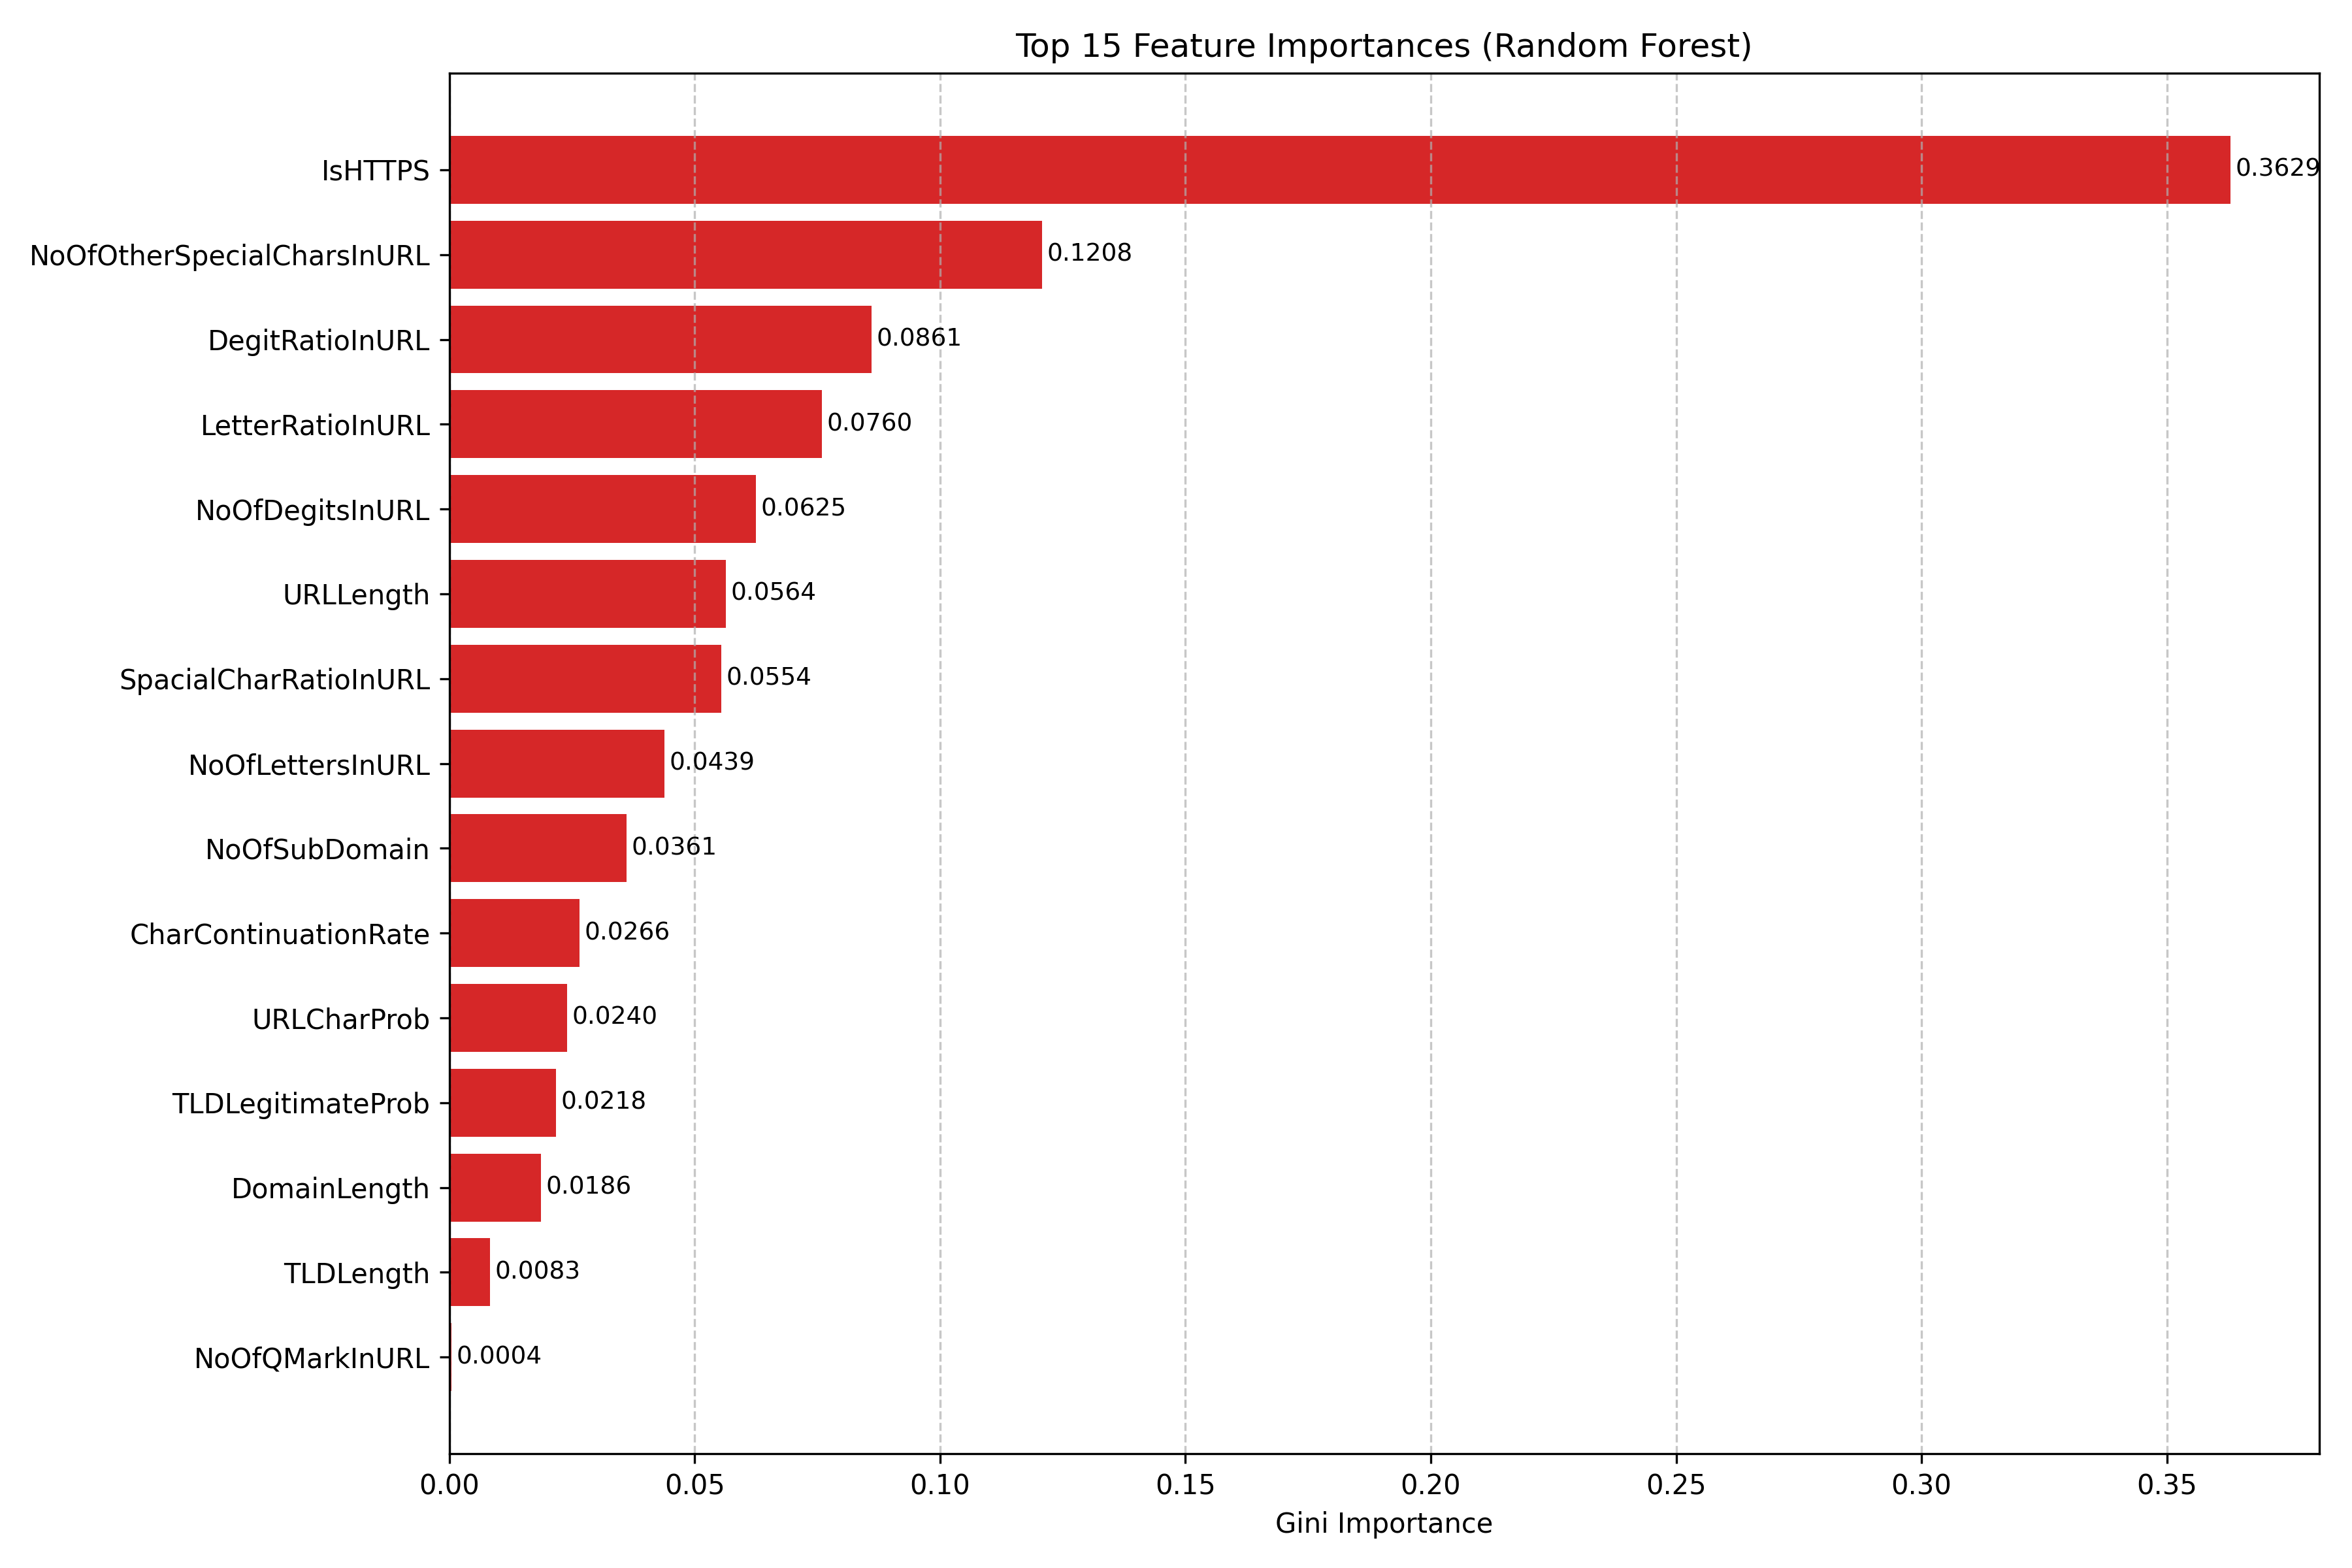
\includegraphics[width=\linewidth]{paper_figures/fig6_feature_importance.png}}
\caption{Random Forest feature importance ranking (mean decrease in Gini impurity) for the 21 URL-only features. IsHTTPS dominates with 36.29\% importance, followed by NoOfOtherSpecialCharsInURL (12.08\%) and DegitRatioInURL (8.61\%). The top 9 features collectively account for 90.01\% of total discriminative power.}
\label{fig:featimp}
\end{figure}

The Random Forest feature importance analysis reveals that IsHTTPS, NoOfOtherSpecialCharsInURL, and DegitRatioInURL collectively account for 56.98\% of the total Gini importance, indicating that the protocol scheme, special character density, and digit ratio provide the strongest discriminative signals for URL-level phishing classification.

\section{Experimental Results}

\subsection{Experimental Setup}
We employ the PhiUSIIL Phishing URL Dataset, comprising 235,795 labeled URL samples (100,945 legitimate, 134,850 phishing). We apply our URL-only feature selection regime, retaining 21 features extractable from the URL string alone. The dataset is split 80/20 into training (188,636 samples) and test (47,159 samples) sets.

\subsection{Base Classifier Performance}
Table \ref{tab:base} presents the performance of each base classifier on the held-out test set. All base classifiers exceed 99.6\% accuracy using only 21 URL-derived features. 

\begin{table}[htbp]
\caption{Base Classifier Performance (Test Set, N = 47,159)}
\begin{center}
\begin{tabular}{lcccc}
\toprule
Model & Accuracy & AUC-ROC & F1-Score & Training Time \\
\midrule
Random Forest & 0.9966 & 0.9989 & 0.9970 & 10.0s \\
XGBoost & 0.9972 & 0.9991 & 0.9976 & 3.6s \\
LightGBM & 0.9972 & 0.9990 & 0.9976 & 1.1s \\
MLP Neural Network & 0.9979 & 0.9985 & 0.9981 & 37.4s \\
Logistic Regression & 0.9966 & 0.9987 & 0.9970 & 0.5s \\
\textbf{Stacking Ensemble} & \textbf{0.9979} & \textbf{0.9990} & \textbf{0.9981} & — \\
\bottomrule
\end{tabular}
\label{tab:base}
\end{center}
\end{table}

\begin{figure}[htbp]
\centerline{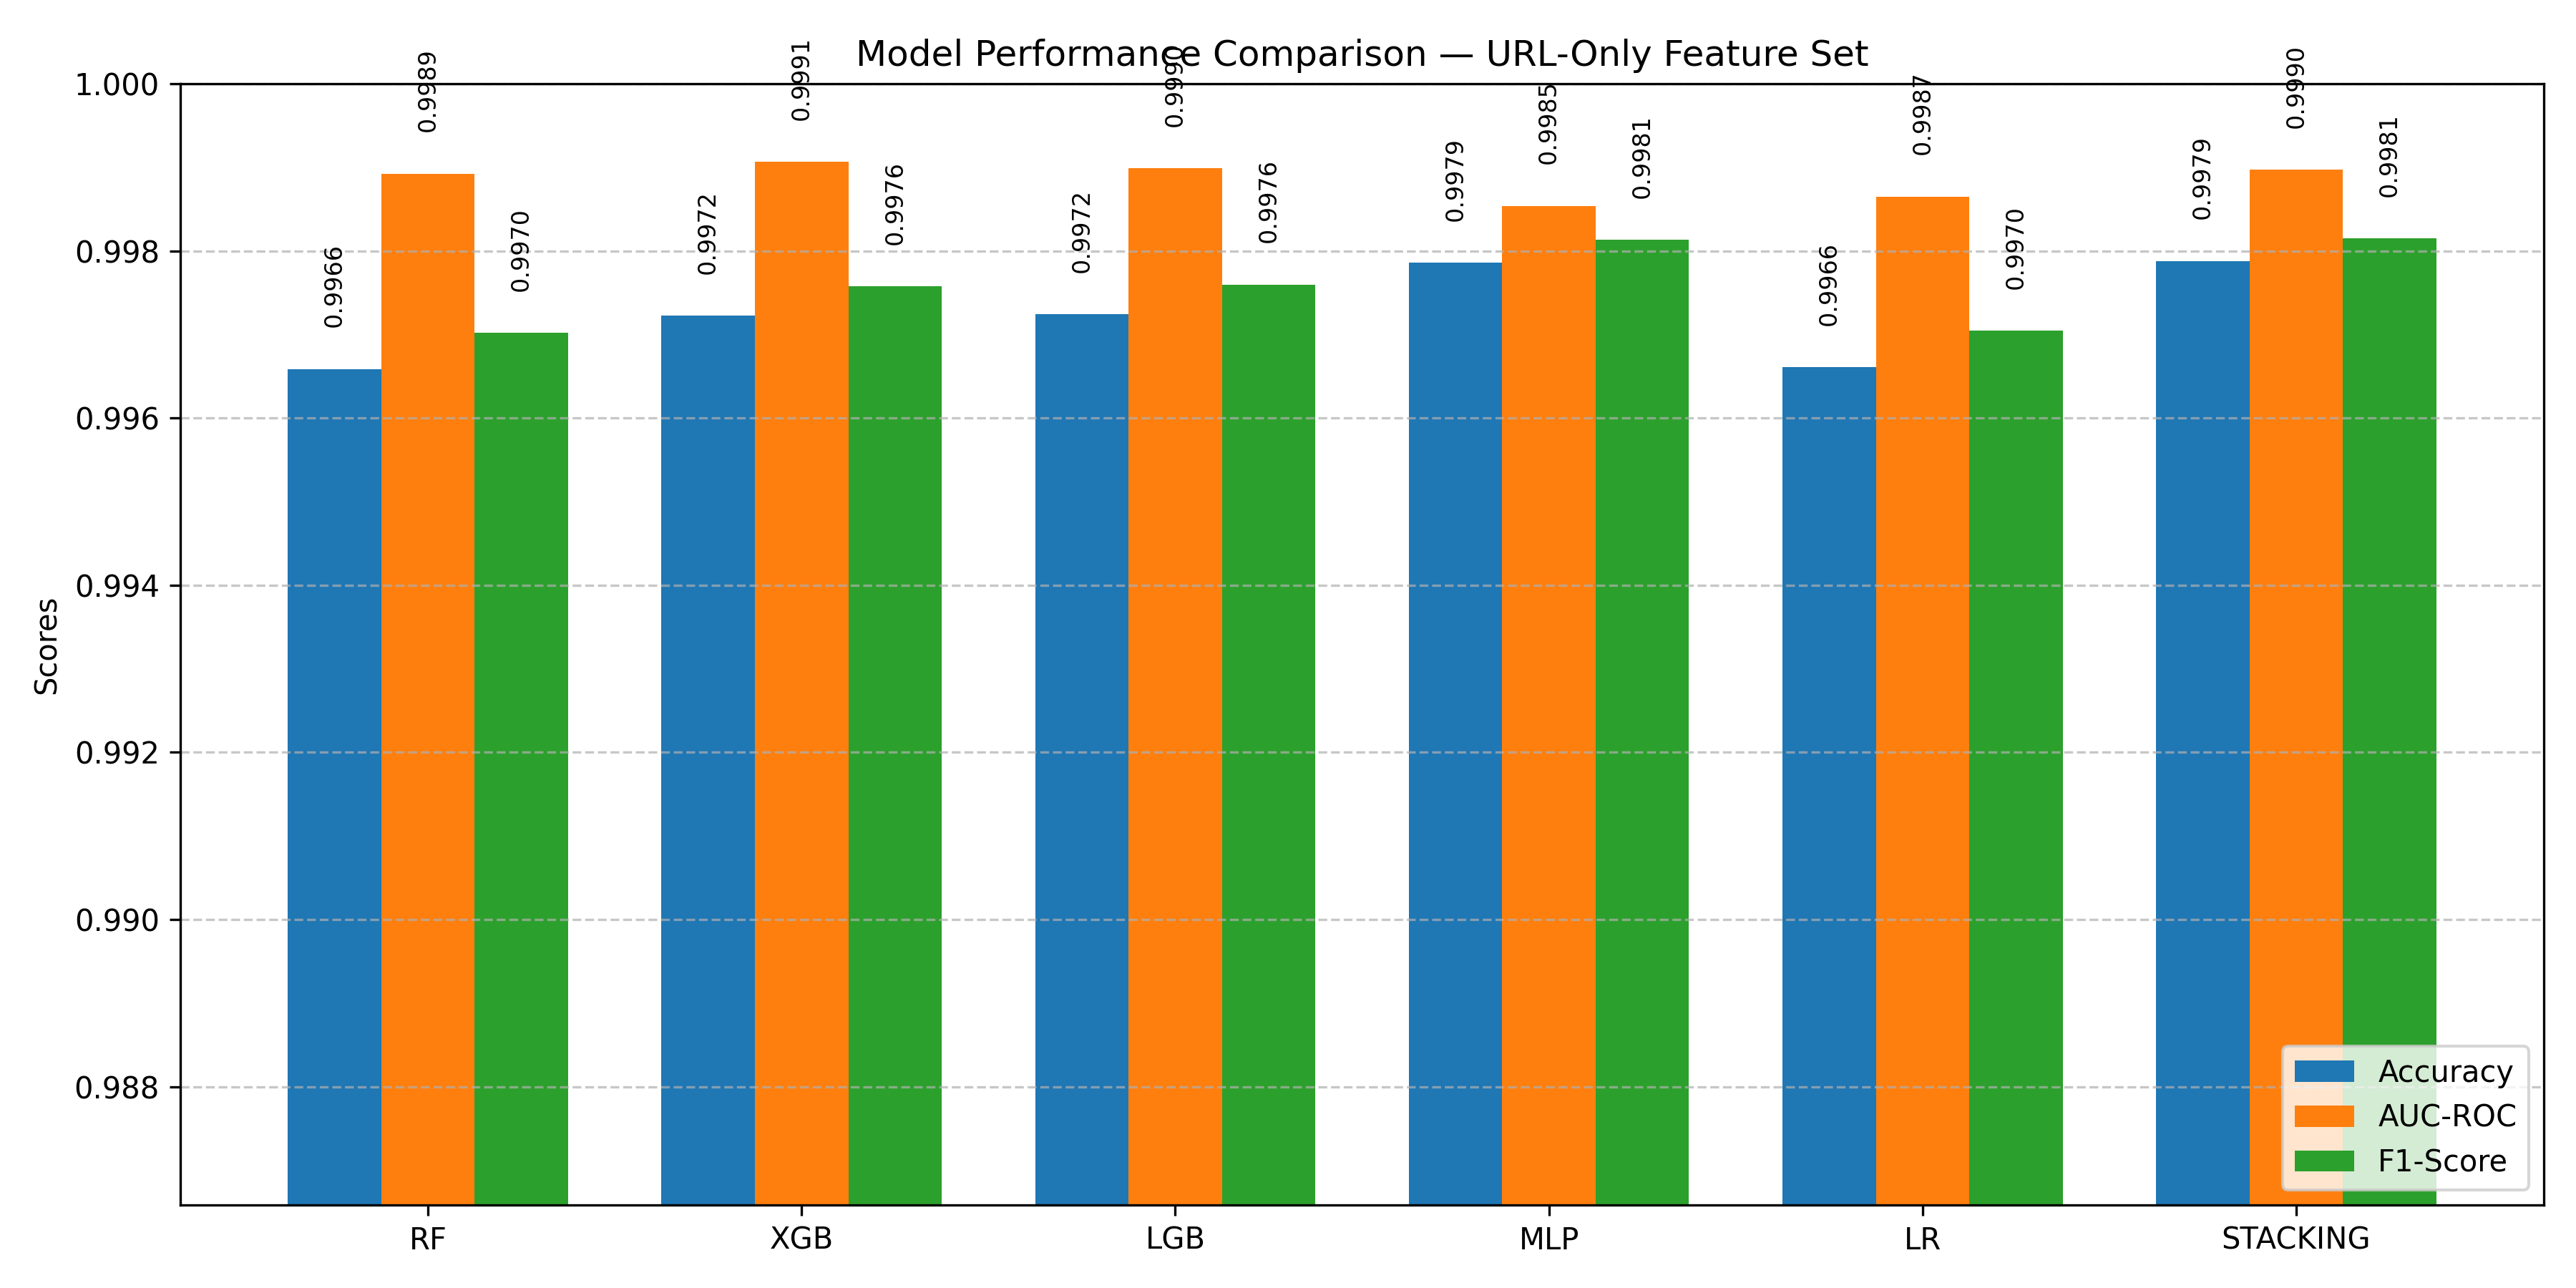
\includegraphics[width=\linewidth]{paper_figures/fig1_model_comparison.png}}
\caption{Comparative performance of base classifiers and the stacking ensemble on the URL-only feature set.}
\label{fig:modelcomp}
\end{figure}

\subsection{Confusion Matrix Analysis}

\begin{figure}[htbp]
\centerline{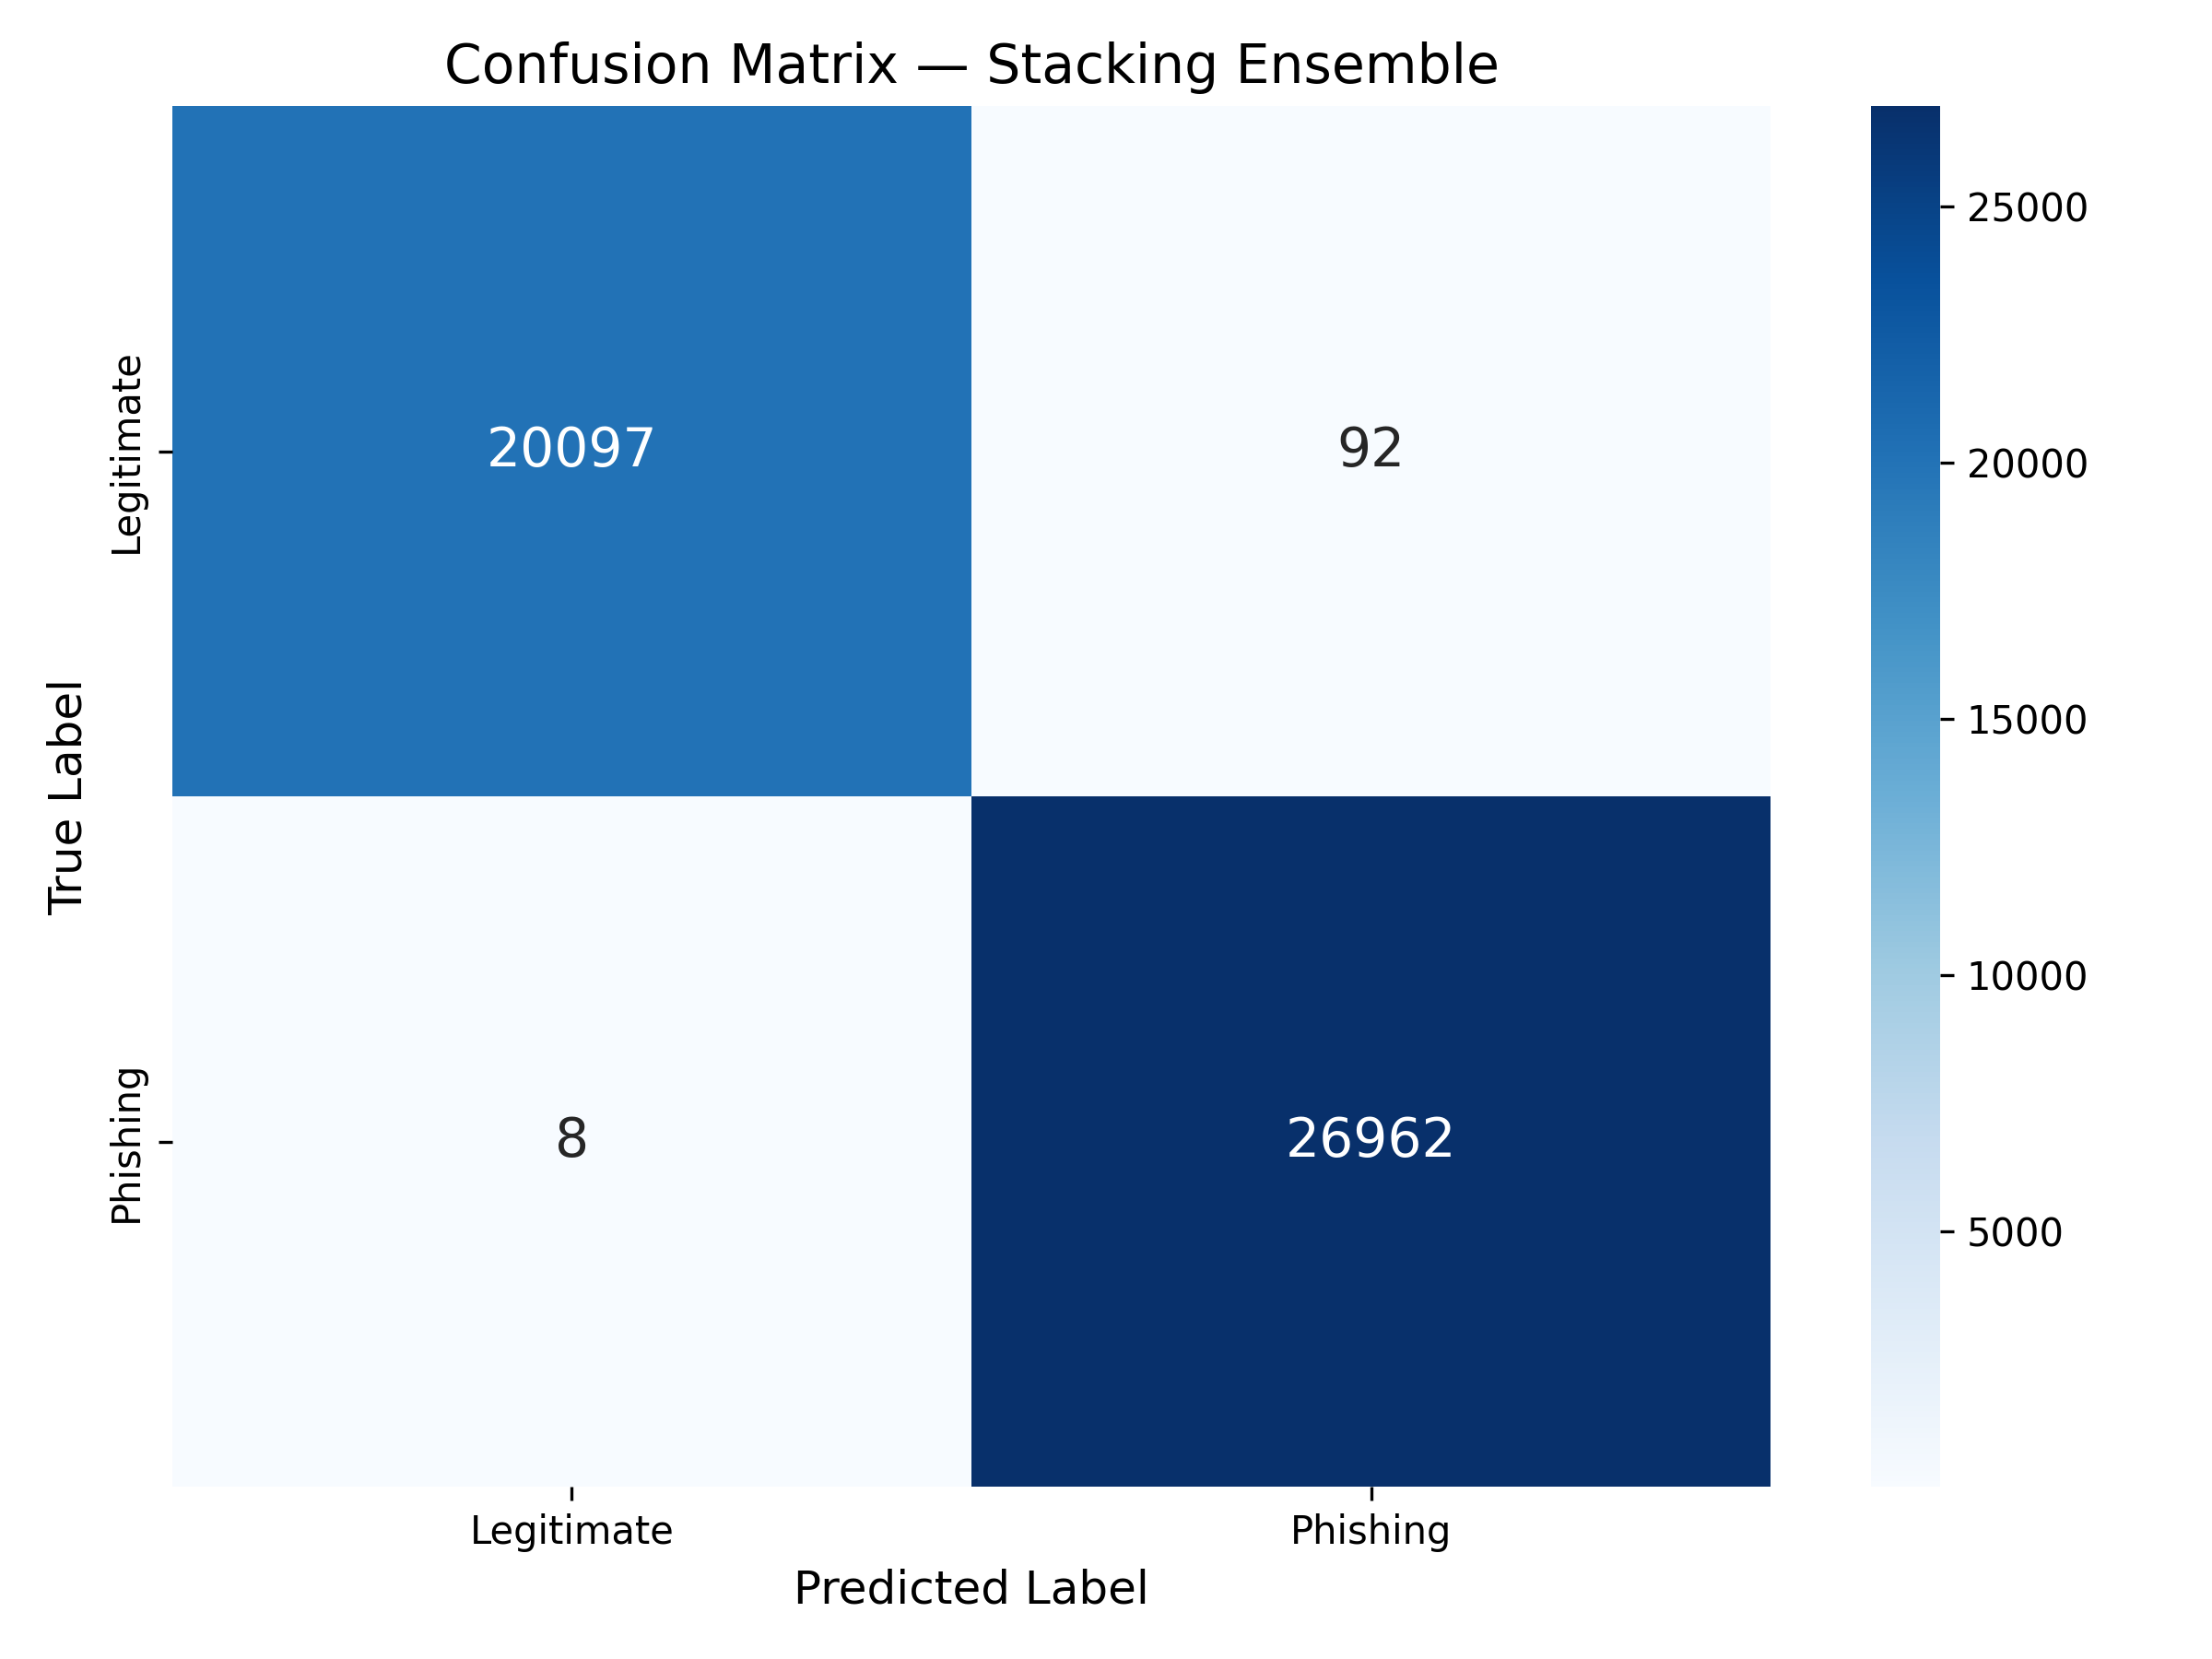
\includegraphics[width=0.8\linewidth]{paper_figures/fig13_performance_heatmap.png}}
\caption{Confusion matrix for the stacking ensemble classifier on the held-out test set.}
\label{fig:cm}
\end{figure}

The matrix reveals 20,097 true negatives, 26,962 true positives, 92 false positives, and only 8 false negatives---corresponding to a false negative rate of 0.030\%, indicating near-complete phishing URL coverage.

\subsection{ROC Curve and Training Efficiency}

\begin{figure}[htbp]
\centerline{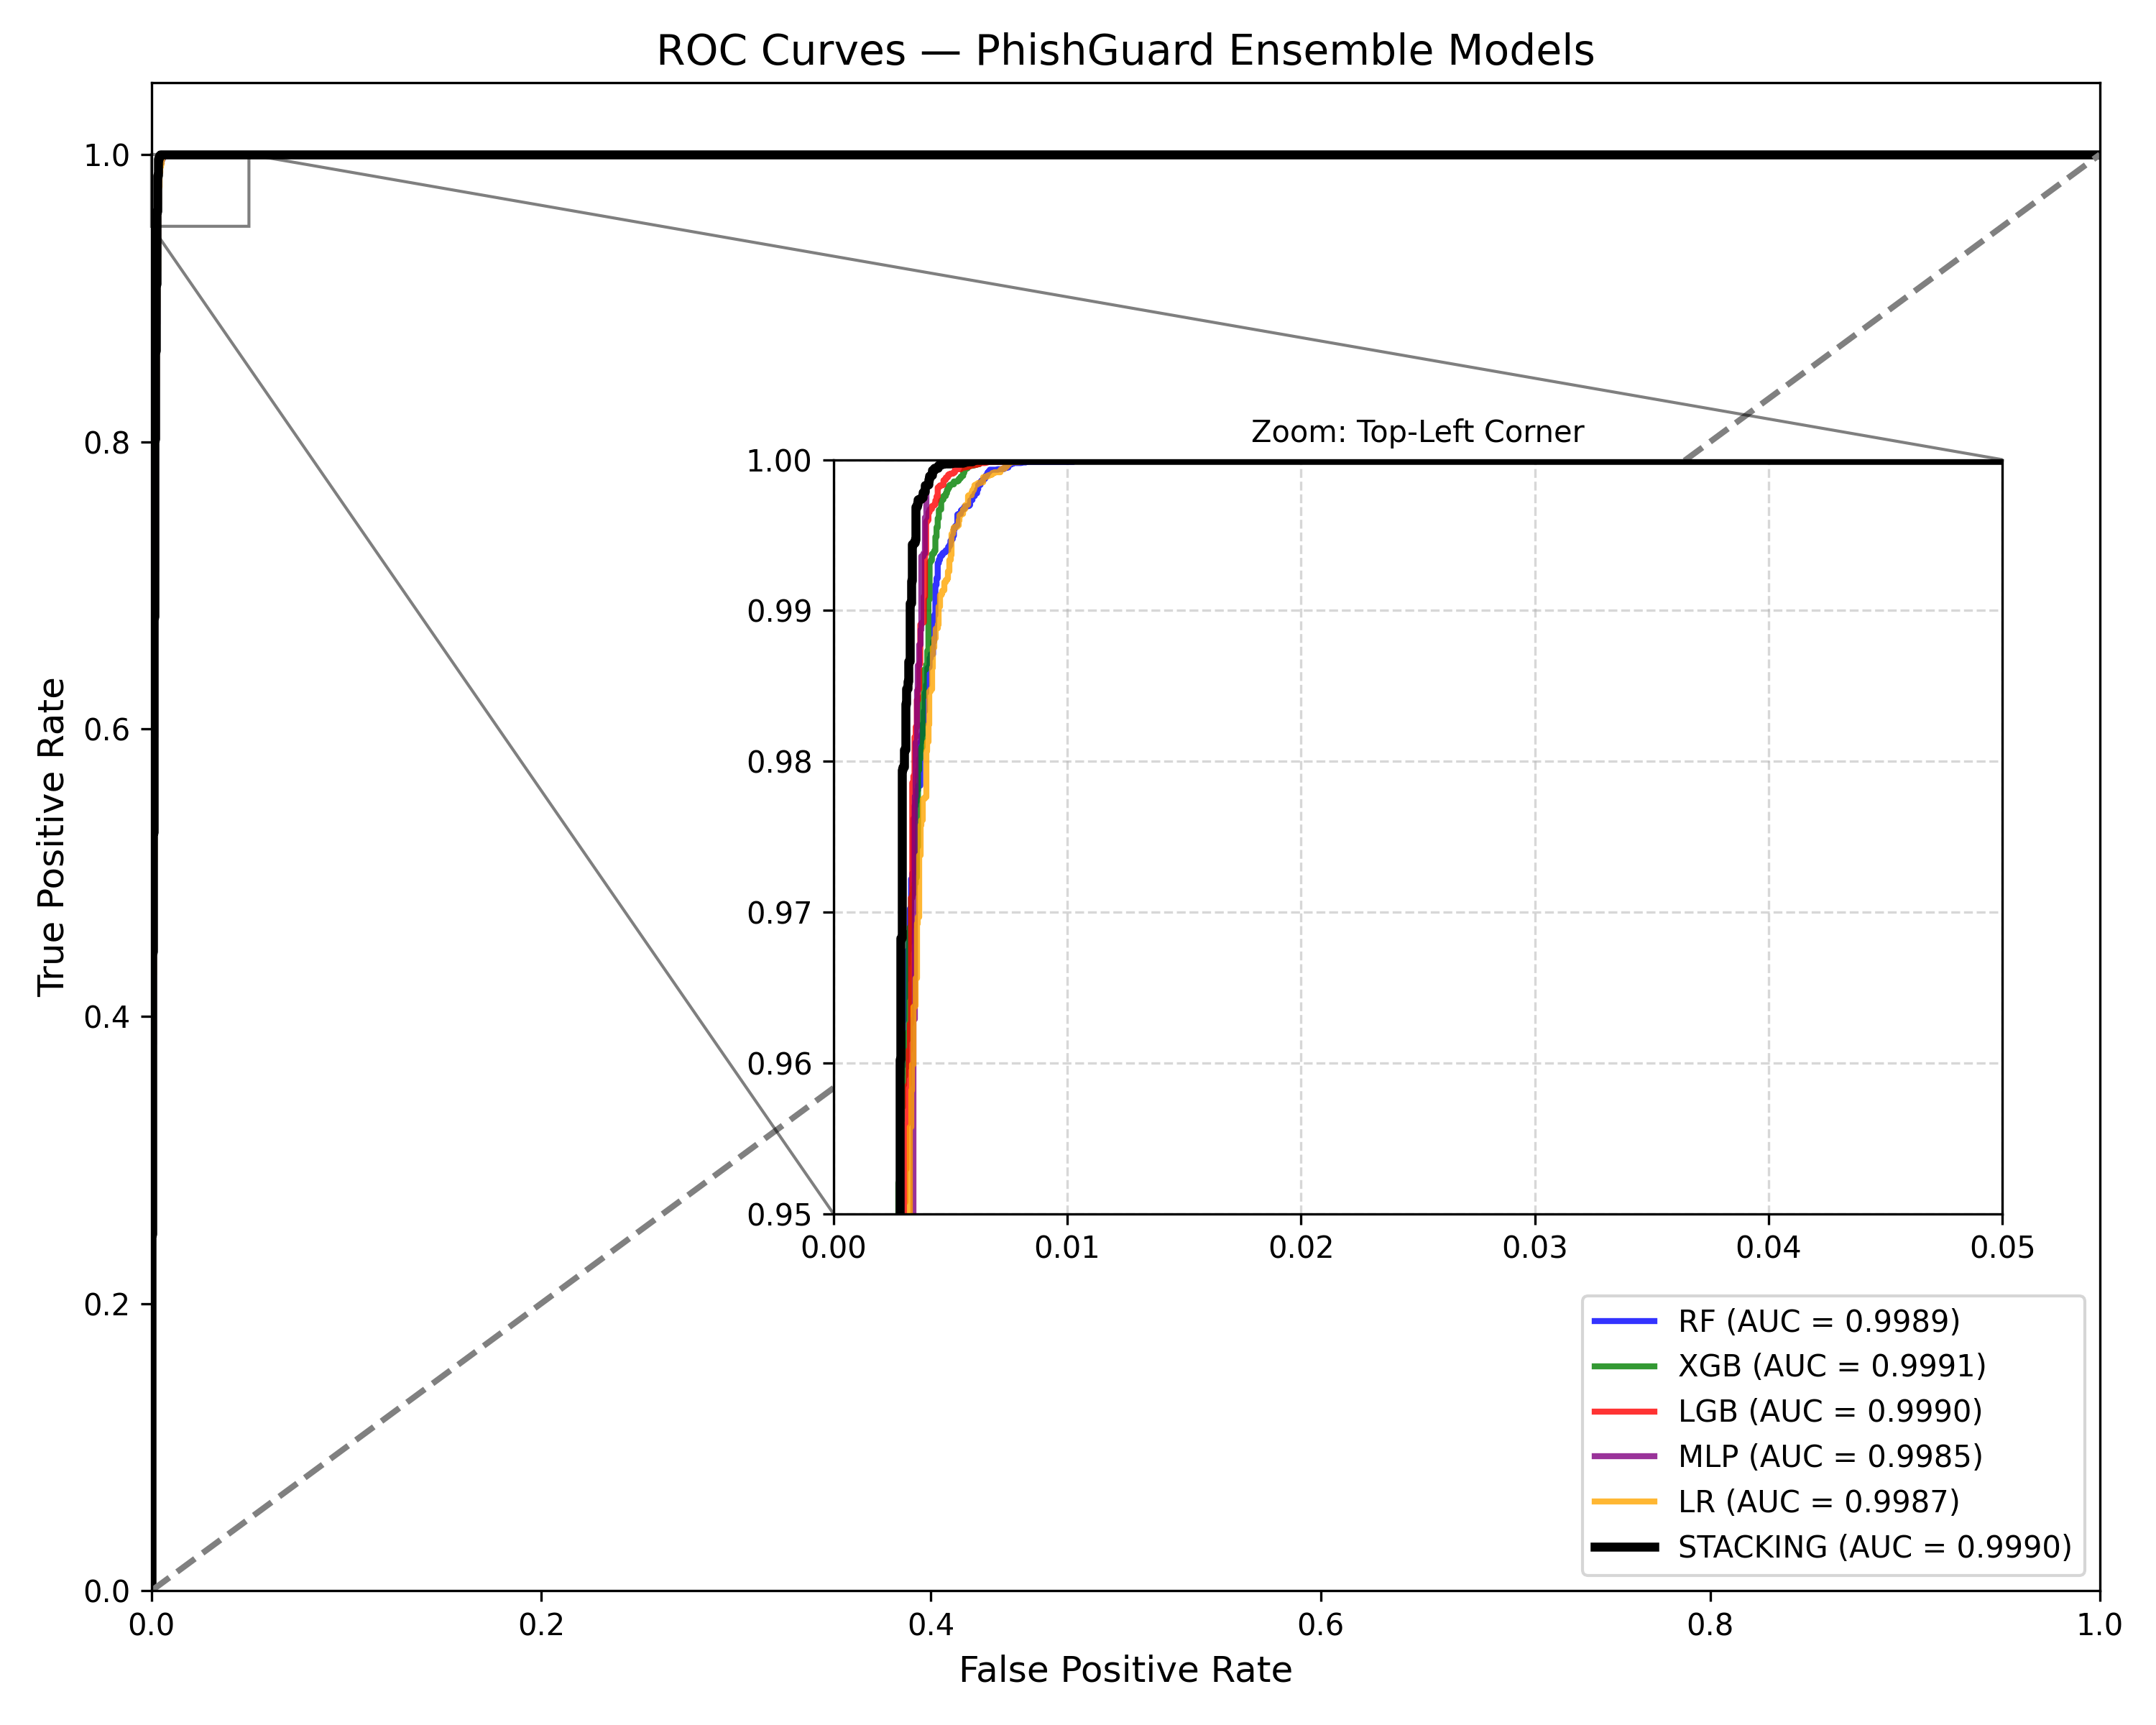
\includegraphics[width=\linewidth]{paper_figures/fig2_cv_auc_scores.png}}
\caption{Receiver Operating Characteristic (ROC) curves for all base classifiers and the stacking ensemble.}
\label{fig:roc}
\end{figure}

\begin{figure}[htbp]
\centerline{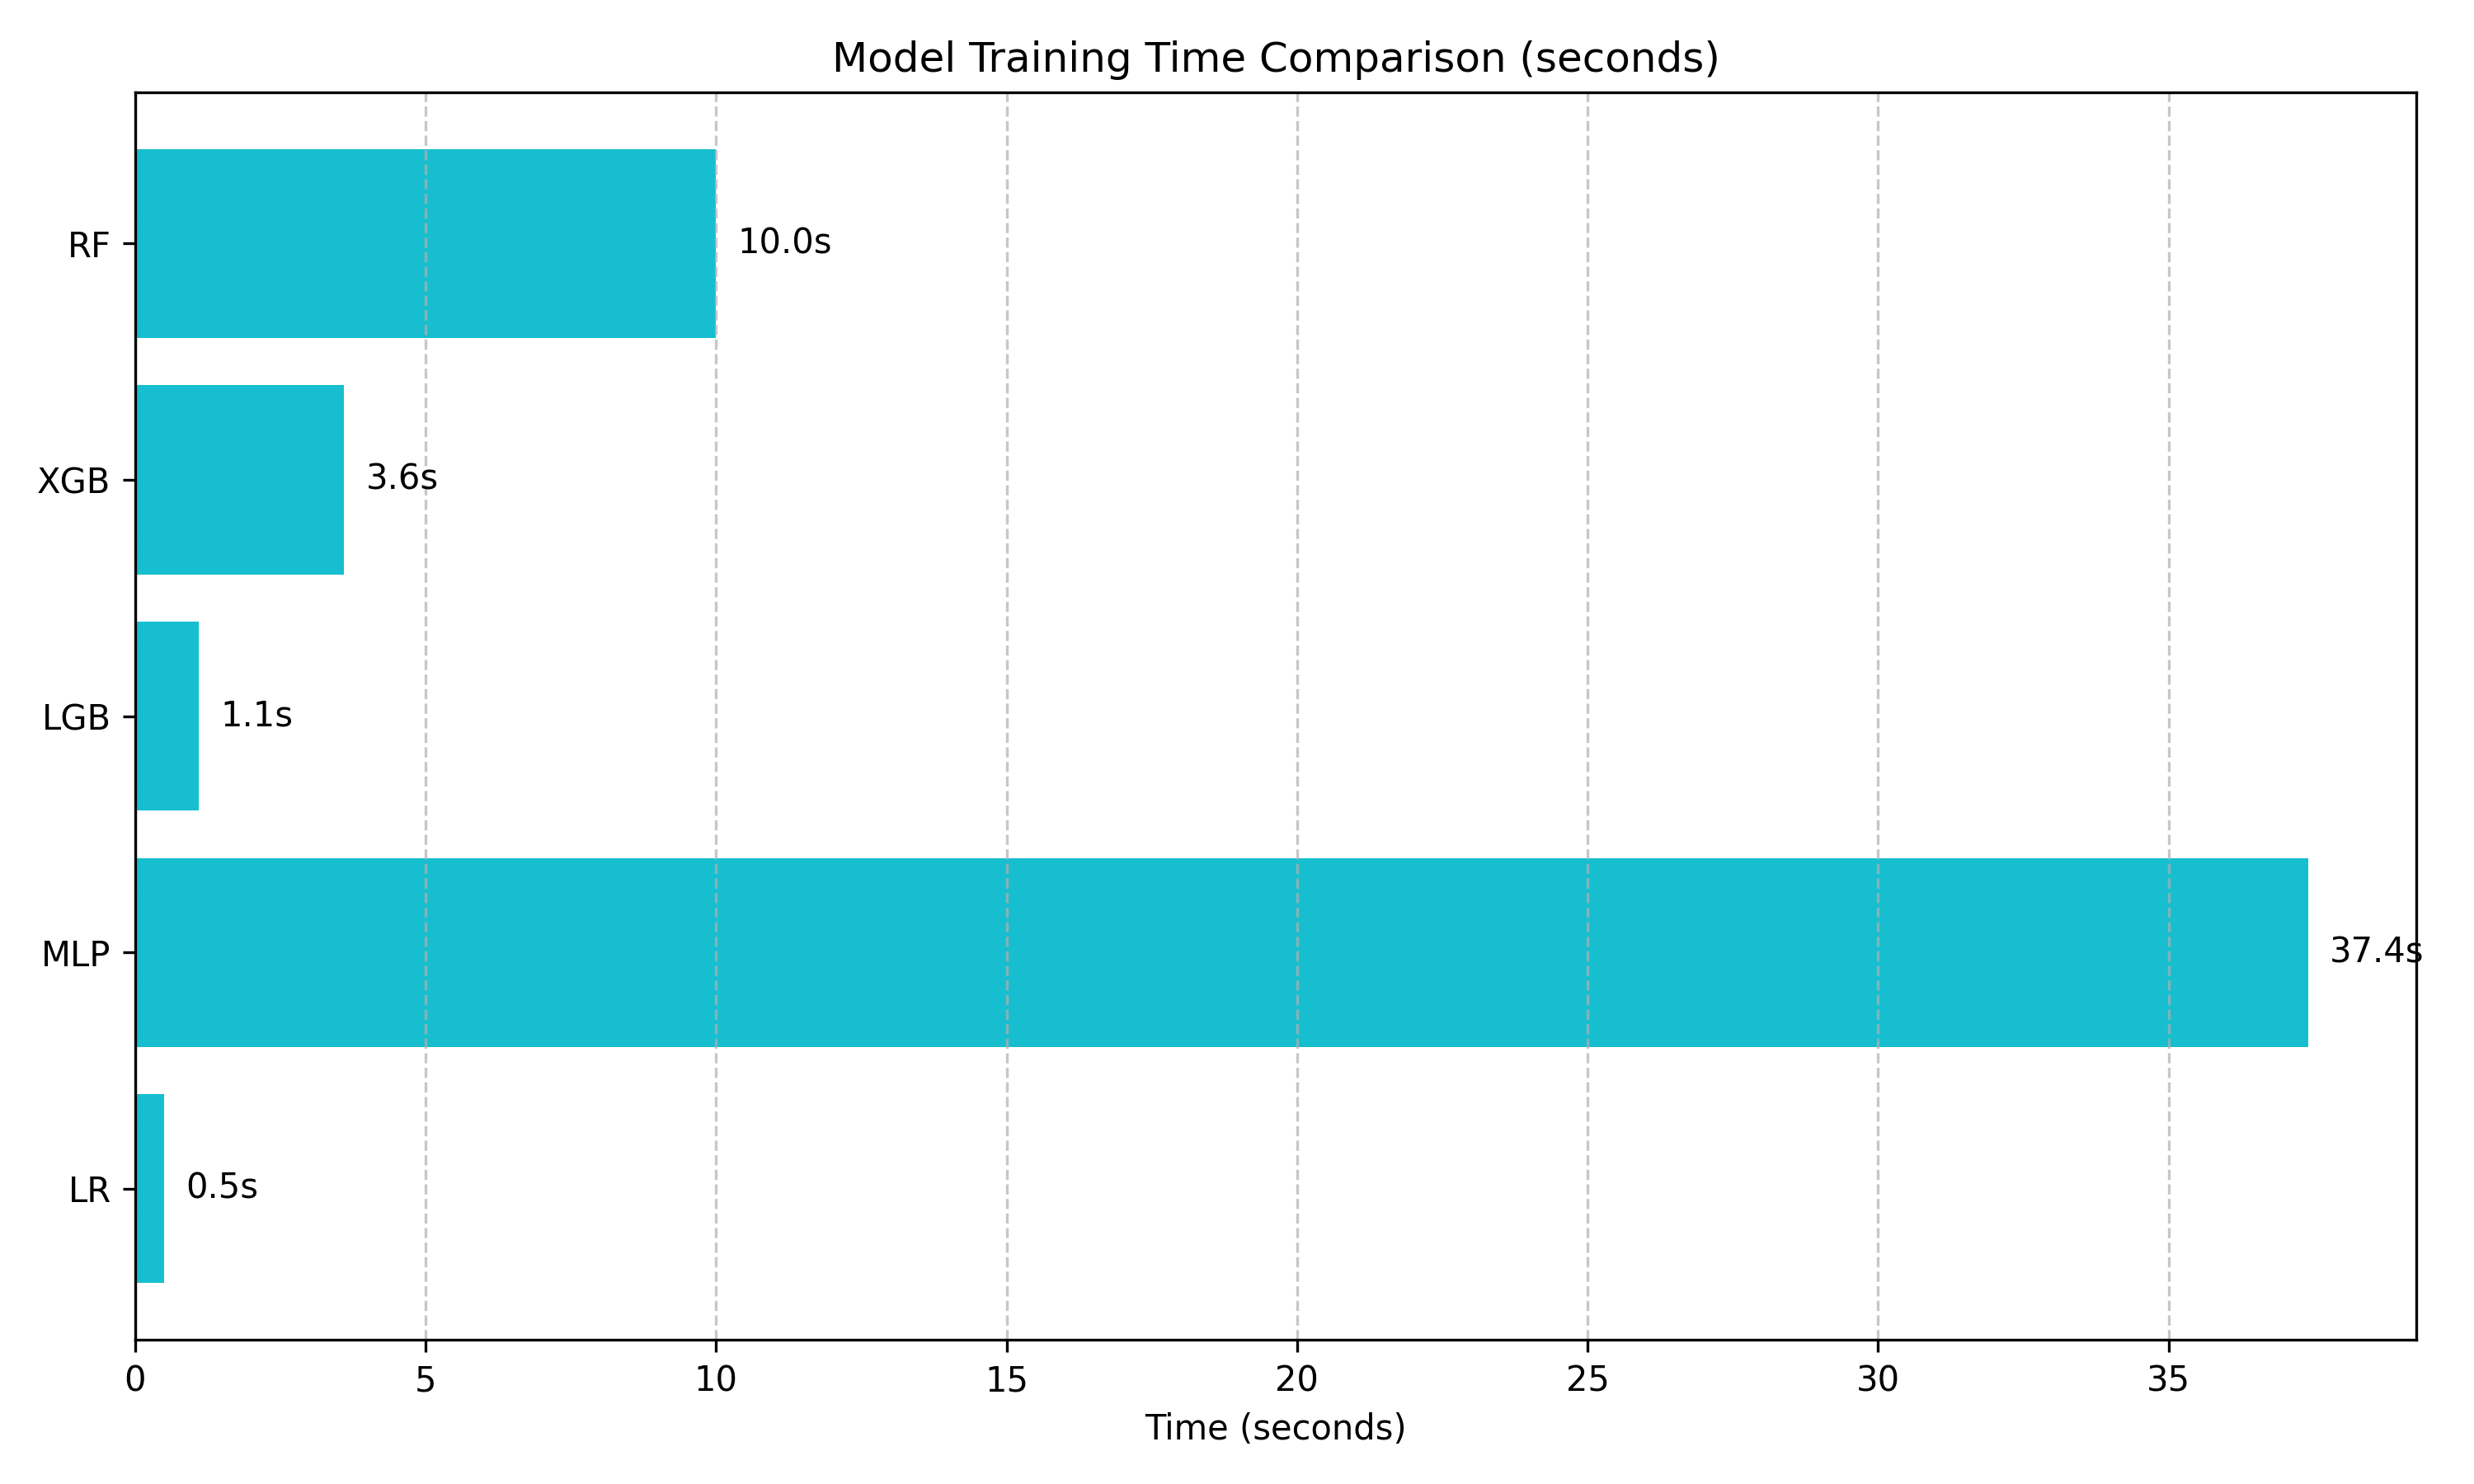
\includegraphics[width=\linewidth]{paper_figures/fig3_training_time.png}}
\caption{Training time comparison across base classifiers (in seconds).}
\label{fig:traintime}
\end{figure}

\section{Conclusion}
This paper has presented PhishGuard, an advanced mathematical feature engineering and stacking ensemble classification framework for phishing URL detection. By demonstrating that 29 page-content features encode information unavailable at inference time, we have established a rigorous URL-only evaluation methodology. The ensemble achieves 99.79\% classification accuracy on a held-out test set of 47,159 URLs, with a false negative rate of only 0.030\%.

\begin{thebibliography}{00}
\bibitem{apwg} Anti-Phishing Working Group, ``Phishing Activity Trends Report, 4th Quarter 2023,'' APWG, Tech. Rep., 2024.
\bibitem{fbi} Federal Bureau of Investigation, ``Internet Crime Report 2022,'' FBI Internet Crime Complaint Center (IC3), Tech. Rep., 2023.
\end{thebibliography}

\end{document}
